\documentclass[aspectratio=169, bigger, xcolor=table]{beamer}
\usepackage[magyar]{babel}
\usepackage{t1enc}
\usepackage{lipsum}

\begin{document}

    \AtBeginSection{\begin{frame}
            \sectionpage
        \end{frame}
        \begin{frame}
    \tableofcontents[currentsection]
\end{frame}}

    \begin{frame}
            \title{Cím dia}
            \subtitle{Cím dia alcíme}
            
            \maketitle
    \end{frame}
    
    \section{1. feladat}
    
        
        \begin{frame}{Cím}{Alcím}
            sima
            \newline
            még pár szó
        \end{frame}
        
        \subsection{1.1 section}
        \begin{frame}[fragile]{Verbatim}
            \begin{verbatim}
                Tétel környezet kódja:
                    Preambulum:
                        \newtheorem{típus}[számozás módja]{név}
                    Document:
                        \begin{típus}
                            Szöveg...
                        \end{típus}
            \end{verbatim}
        \end{frame}
        
        \subsection{1.2 section}
        \begin{frame}[allowframebreaks]{Tördelt}
            \lipsum[2-5]
        \end{frame}
    
    \section{2. feladat}
        
        \subsection{2.1 section}
        \begin{frame}{Oszlopok}
            \begin{columns}[t]
                \begin{column}{.5\linewidth}
                    \begin{itemize}
                        \item pont
                        \item pontpont
                    \end{itemize}
                    
                    \begin{enumerate}
                        \item első
                        \item második
                        \item harmadik
                    \end{enumerate}
                \end{column}
                
                \begin{column}{.5\linewidth}
                    \begin{figure}
                        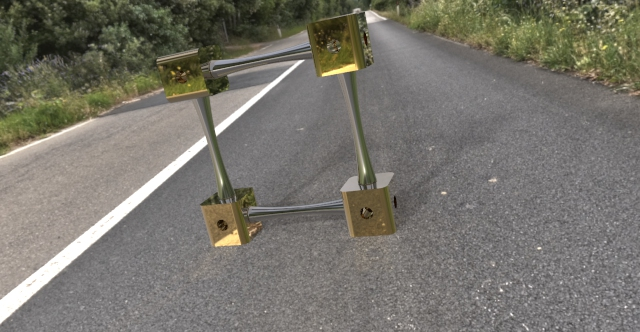
\includegraphics[keepaspectratio, width=5cm]{8. Lesson/creo.jpg}
                        \caption{Kép}
                    \end{figure}
                \end{column}
            \end{columns}
        \end{frame}
        
        \subsection{2.2 section}
        \begin{frame}{Blokkok}
            \begin{block}
                cím nélkül
            \end{block}
            
            \begin{block}{sima}
                kék
            \end{block}
            
            \begin{exampleblock}{példa}
                zöld
            \end{exampleblock}
            
            \begin{alertblock}{figyelmeztető}
                piros
            \end{alertblock}
        \end{frame}
        
        \subsection{2.3 section}
        \begin{frame}{Theorem, proof}
            \begin{theorem}
                Pitagorasz tétele...
            \end{theorem}
            
            \begin{proof}[Pitagorasz tétel bizonyítása]
                Készítsünk két darab... \qedhere
            \end{proof}
        \end{frame}
        
        \subsection{2.4 section}
        \begin{frame}{Semiverbatim}
            \begin{semiverbatim}
                Lista kódja:
                
                    \\begin\{enumerate\}
                    
                        \textcolor{red}{\\item egy}
                        
                        \\begin\{itemize\}
                        
                            \textcolor{blue}{\\item második szint}
                            
                        \\end\{itemize\}
                        
                        \\item kettő
                        
                    \\end\{enumerate\}
            \end{semiverbatim}
        \end{frame}
    
\end{document}